\chapter{Policy Gradient Avanzado}

\lecture{9}{2020-06-17}{Advanced Policy Gradient}

\section{¿Por qué los métodos Policy Gradient funcionan?}%
\label{sec:_por_qué_los_métodos_policy_gradient_funcionan_}

Una vista de alto nivel de los algoritmos Policy Gradient es la ejecución en bucle de estos dos
pasos:
\begin{enumerate}
    \item Estimar $\hat{A}^\pi(s_t,a_t)$ para la política $\pi$ actual.
    \item Usar $\hat{A}^\pi(s_t,a_t)$ para obtener una política mejorada $\pi'$.
\end{enumerate}

Esto es similar al algoritmo de iteración de política (\textit{Policy Iteration
Algorithm}):
\begin{enumerate}
    \item Evaluar $A^\pi(s,a)$.
    \item $\pi\gets\pi'$
\end{enumerate}

Por lo que se puede enmarcar Policy Gradient dentro de Policy Iteration.

\section{Policy Gradient es un tipo de iteración de política}%
\label{sec:policy_gradient_es_un_tipo_de_iteración_de_política}

Siendo:
\begin{align}
J ( \theta ) = E _ { \tau \sim p _ { \theta } ( \tau ) } \left[ \sum _ { t } \gamma ^ { t } r ( s
    _ { t } , a _ { t } ) \right]
\end{align}

Se analiza la mejora del objetivo de la política (diferencia entre dos políticas)
($\theta'$ es lo que se busca y $\theta$ es la política que ya se tiene). 

\begin{align}
    J(\theta') - J(\theta) &=
    J(\theta')-E_{s_0\sim p(s_0)}[V^{\pi_\theta}(s_0)]\\
    &=J(\theta')-E_{\tau\sim p(\tau)}[V^{\pi_\theta}(s_0)] \textrm{ ya que las trayectorias
    empiezan en } s_0\\
    &= J ( \theta ^ { \prime } ) - E _ { \tau \sim p _ { \theta ^ { \prime } } ( \tau ) } \left[
        \sum _ { t = 0 } ^ { \infty } \gamma ^ { t } V ^ { \pi _ { \theta } } ( s _ { t } ) -
        \sum _ { t = 1 } ^ { \infty } \gamma ^ { t } V ^ { \pi _ { \theta } } ( s _ { t } )
    \right]\\
    &= J ( \theta ^ { \prime } ) + E _ { \tau \sim p _ { \theta ^ { \prime } } ( \tau ) } \left[
        \sum _ { t = 0 } ^ { \infty } \gamma ^ { t } ( \gamma V ^ { \pi _ { \theta } } ( s _ { t
        + 1 } ) - V ^ { \pi _ { \theta } } ( s _ { t } ) ) \right]\\
    &= E _ { \tau \sim p _ { \theta ^ { \prime } } ( \tau ) } \left[ \sum _ { t = 0 } ^ { \infty
        } \gamma ^ { t } r ( s _ { t } , a _ { t } ) \right] + E _ { \tau \sim p _ { \theta ^ { \prime
    } } ( \tau ) } \left[ \sum _ { t = 0 } ^ { \infty } \gamma ^ { t } ( \gamma V ^ { \pi _ {
    \theta } } ( s _ { t + 1 } ) - V ^ { \pi _ { \theta } } ( s _ { t } ) ) \right]\\
&=E _ { \tau \sim p _ { \theta ^ { \prime } } ( \tau ) } \left[ \sum _ { t = 0 } ^ { \infty }
    \gamma ^ { t } ( r ( s _ { t } , a _ { t } ) + \gamma V ^ { \pi _ { \theta } } ( s _ { t + 1
    } ) - V ^ { \pi _ { \theta } } ( s _ { t } ) ) \right]\\
&= E _ { \tau \sim p _ { \theta ^ { \prime } } ( \tau ) } \left[ \sum _ { t = 0 } ^ { \infty }
\gamma ^ { t } A ^ { \pi _ { \theta } } ( s _ { t } , a _ { t } )\right]
\end{align}

Se intenta optimizar esto más, ya que la esperanza está con respecto a $\pi_{\theta'}$. Es
muy difícil calcular los gradientes de esta forma desde nuestras muestras, porque la esperanza
es con respecto a $\pi_{\theta'}$ y el \textit{advantage} se calcula con $\pi_\theta$. Se
puede hacer lo siguiente:

\begin{align}
E _ { \tau \sim p _ { \theta ^ { \prime } } ( \tau ) } \left[ \sum _ { t } \gamma ^ { t } A ^ {
    \pi _ { \theta } } ( s _ { t } , a _ { t } ) \right] = \sum _ { t } E _ { s _ { t } \sim p _ { \theta ^ { \prime } } ( s _ { t } ) } [ E _ { a _ { t } \sim \pi _ { \theta ^ { \prime } } ( a _ { t } | s _ { t } ) } [ \gamma ^ { t } A ^ { \pi _ { \theta } } ( s _ { t } , a _ { t } ) ] ]
\end{align}

Si se tiene una esperanza de una suma se puede sacar la suma fuera, quedando dentro la suma se la
esperanza con respecto al \textit{state-marginal} $p_{\theta'}$ de la acción con respecto a
$\pi_{\theta'}$ del \textit{advantage}. A continuación se usa el mismo truco usado en el tema 3
para llevar a cabo Importance Sampling:

\begin{align*}
    E_{x\sim p (x)}[f(x)] &= \int p(x)f(x)dx\\
                          &=\int \frac{q(x)}{q(x)} p(x)f(x)dx\\
                          &=\int q(x) \frac{p(x)}{q(x)} f(x)dx\\
                          &=E_{x\sim q(x)}\left[ \frac{p(x)}{q(x)} f(x)\right]
\end{align*}

Por lo que la ecuación anterior queda como:
\begin{align}
E _ { \tau \sim p _ { \theta ^ { \prime } } ( \tau ) } \left[ \sum _ { t } \gamma ^ { t } A ^ {
    \pi _ { \theta } } ( s _ { t } , a _ { t } ) \right] 
&= \sum _ { t } E _ { s _ { t } \sim p _ { \theta ^ { \prime } } ( s _ { t } ) } \left[ E _ { a _
    { t } \sim \pi _ { \theta } ( a _ { t } | s _ { t } ) } \left[ \frac { \pi _ { \theta ^ {
    \prime } } ( a _ { t } | s _ { t } ) } { \pi _ { \theta } ( a _ { t } | s _ { t } ) } \gamma
    ^ { t } A ^ { \pi _ { \theta } } ( s _ { t } , a _ { t } ) \right] \right]
\end{align}

Todavía se tiene un problema que impide optimizar el problema: se tiene $\theta'$ en la
esperanza exterior. Lo que nos impide usar $\pi_\theta$ para crear las muestras. ¿Se podría
cambiar  $p_{\theta'}$
por $p_{\theta}$ sin que pasase nada (que fuesen lo suficientemente similares)? Si esto
fuera cierto, se cumpliría que:
\begin{align}
    \label{eq:tema7loqueseintentademostrar}
    J(\theta') - J(\theta) \approx \bar{A}(\theta') \implies \theta'\gets
    arg\max_{\theta'} \bar{A}(\theta)
\end{align}
Donde:
\begin{align}
    \bar{A}(\theta') = 
\sum _ { t } E _ { s _ { t } \sim p _ { \theta ^ { \prime } } ( s _ { t } ) } \left[ E _ { a _
    { t } \sim \pi _ { \theta } ( a _ { t } | s _ { t } ) } \left[ \frac { \pi _ { \theta ^ {
    \prime } } ( a _ { t } | s _ { t } ) } { \pi _ { \theta } ( a _ { t } | s _ { t } ) } \gamma
    ^ { t } A ^ { \pi _ { \theta } } ( s _ { t } , a _ { t } ) \right] \right]
\end{align}

Se pueden calcular los gradientes de $\bar{A}(\theta')$ sin generar ninguna muestra más. Este
paso sería el quivalente al paso 2 de \textit{policy iteration}. 

¿Esto es verdad? ¿Y si es así, cuándo? Se va a intentar demostrar la afirmación de que
$p_\theta (s_t)$ se acerca a  $p_{\theta'}(s_t)$ cuando  $\pi_\theta$ se está cerca de
$\pi_{\theta'}$. 

En el caso sencillo, se asume que $\pi_\theta$ es una política determinista
$a_t=\pi_\theta(s_t)$. Se dice que una política está cerca de otra si la probabilidad de
escoger una acción diferente de la otra es menor que un número pequeño  $\epsilon$:
 \begin{align}
\pi _ { \theta ^ { \prime } } ( a _ { t } \neq \pi _ { \theta } ( s _ { t } ) | s _ { t } ) \leq \epsilon
\end{align}

Esta definición se usó al principio del curso en Imitation Learning. Donde se usó la expresión:
\begin{align}
p _ { \theta ^ { \prime } } ( s _ { t } ) = ( 1 - \epsilon ) ^ { t } p _ { \theta } ( s _ { t } ) + ( 1 - ( 1 - \epsilon ) ^ { t } ) ) p _ { \text {mistake} } ( s _ { t } )
\end{align}
Se puede acotar la divergencia de la variación total (\textit{total variation divergence})
entre $\pi_{\theta'}$ y  $\pi_\theta$ como:
\begin{align}
    \label{eq:totvaldivaplicada}
| p _ { \theta ^ { \prime } } ( s _ { t } ) - p _ { \theta } ( s _ { t } ) | = ( 1 - ( 1 - \epsilon ) ^ { t } ) | p _ { \text { mistake } } ( s _ { t } ) - p _ { \theta } ( s _ { t } ) |
\end{align}

La divergencia de la variación total se define de la siguiente forma, y se puede pensar en ella
como la distancia entre dos distribuciones de probabilidad:
\begin{align}
    |p_{\theta'}(s_t)-p_\theta(s_t)|=\sum_{s_t}|p_{\theta'}(s_t)-p_\theta(s_t)|
\end{align}

La ecuación \ref{eq:totvaldivaplicada} está acotada de la siguiente manera:
\begin{align}
    \label{eq:totvaldivaplicada}
| p _ { \theta ^ { \prime } } ( s _ { t } ) - p _ { \theta } ( s _ { t } ) | = ( 1 - ( 1 -
\epsilon ) ^ { t } ) | p _ { \text { mistake } } ( s _ { t } ) - p _ { \theta } ( s _ { t } ) |
\leq 2 (1-(1-\epsilon)^t)
\end{align}
Ya que el máximo valor que puede tomar la diferencia absoluta entre dos distribuciones es 2
(porque las distribuciones van de 0 a 1). Para simplificar, se usa la identidad:
$(1-\epsilon)^t \geq 1 - \epsilon t \;\forall \;\epsilon \in [0,1]$. De esta manera se acota por
$\leq 2\epsilon t$. No es una gran acotación, ya que crece linealmente, pero sirve.

Esto es para el caso de usar una política determinista. Se quiere acotar par el caso en que se
use una política estocástica (lo más común). Para ello, hay que definir de otra forma la noción
de cercanía entre dos políticas. Para ello se vuelve a usar la divergencia de variación total.
\begin{align}
\pi _ { \theta ^ { \prime } } \text { es próxima a } \pi _ { \theta } \text { si } | \pi _ {
\theta ^ { \prime } } ( a _ { t } | s _ { t } ) - \pi _ { \theta } ( a _ { t } | s _ { t } ) |
\leq \epsilon \text { para todo } s _ { t }
\end{align}

Esta definición es la misma que la anterior en el caso de políticas deterministas, por
lo que esta es la generalización.

Para poder realizar la derivación a partir de aquí como se hizo para el caso determinista, se usa
el siguiente lema:
\begin{align}
    \text{si }| p _ { X } ( x ) - p _ { Y } ( x ) | = \epsilon , \text { existe } p ( x , y )
    \text { tal que } p ( x ) = p _ { X } ( x ) \text { y } p ( y ) = p _ { Y } ( y ) \text { y }
    p ( x = y ) = 1-\epsilon
\end{align}
Al crear una probabilidad conjunta a partir de dos distribuciones hay infinitas maneras de
hacerlo, pero existe una de ellas en la que se cumple que $x=y$ con probabilidad
$\epsilon$. De este lema se concluye que:
\begin{itemize}
    \item $p_X(x)$ 'coincide' con $p_Y(y)$ con probabilidad $\epsilon$.
    \item $\pi_{\theta'}(a_t|s_t)$ toma una acción diferente de $\pi_\theta(a_t|s_t)$ 
        con probabilidad $\epsilon$ como máximo (si se usan los mismos números aleatorios).
\end{itemize}

Para un análisis más detallado mirar la publicación \textit{Trust Region Policy Optimization}
de Schulman et.al.

Con esto se puede aplicar al caso estocástico el mismo análisis que en el caso determinista,
por lo que se obtiene el mismo resultado que en la ecuación \ref{eq:totvaldivaplicada} y
queda acotada por $2\epsilon t$ de nuevo. Por lo que los \textit{state-marginals} también
serán parecidos.

Sabiendo esto, se intenta demostrar la ecuación
\ref{eq:tema7loqueseintentademostrar}. Para ello se intenta derivar una expresión general de
lo anterior para meterla en la demostración.

\begin{align}
    \sum_{s_t}p_{\theta'}(s_t)f(s_t)&=\sum_{s_t}(p_{\theta'}(s+t)+p+\theta(s_t)-p_\theta(s_t))f(s_t)\\
&=\sum_{s_t}p_\theta(s_t)f(s_t)+(p_{\theta'}(s_t)-p_\theta(s_t))f(s_t)\\
&\geq\sum_{s_t}p_\theta(s_t)f(s_t)+|p_{\theta'}(s_t)-p_\theta(s_t)|f(s_t)\\
&=\sum_{s_t}p_\theta(s_t)f(s_t)+|p_{\theta'}(s_t)-p_\theta(s_t)|\max_{s_t}f(s_t)\\
&\geq E_{p_\theta(s_t)}\left[f(s_t)\right]-2\epsilon t \max_{s_t} f(s_t)
\end{align}

Si $\epsilon$ es un valor muy pequeño, el segundo término puede ser insignificante.

Habiendo derivado esto, se mete en la ecuación \ref{eq:totvaldivaplicada} y se obtiene:
\begin{align}
\sum _ { t } E _ { s _ { t } \sim p _ { \theta ^ { \prime } } ( s _ { t } ) } \left[ E _ { a _ { t }
\sim \pi _ { \theta } ( a _ { t } | s _ { t } ) } \left[ \frac { \pi _ { \theta ^ { \prime } } ( a _ {
t } | s _ { t } ) } { \pi _ { \theta } ( a _ { t } | s _ { t } ) } \gamma ^ { t } A ^ { \pi _ {
\theta } } ( s _ { t } , a _ { t } ) \right] \right] &\geq\\
\sum _ { t } E _ { s _ { t } \sim p _ { \theta } ( s _ { t } ) } \left[ E _ { a _ { t } \sim \pi _ {
\theta } ( a _ { t } | s _ { t } ) } \left[ \frac { \pi _ { \theta ^ { \prime } } ( a _ { t } | s _ {
t } ) } { \pi _ { \theta } ( a _ { t } | s _ { t } ) } \gamma ^ { t } A ^ { \pi _ { \theta } } (
s _ { t } , a _ { t } ) \right] \right] &- \sum _ { t } 2 \epsilon t C
\end{align}

La constante $C$ viene del término $\max_{s_t}f(s_t)$. Este valor se corresponde con el
mayor  \textit{advantage} que se puede obtener, que es la mayor recompensa que se puede recibir
del entorno multiplicada por el número de pasos hasta acabar el episodio. Por lo que la
constante está en el orden de $O(Tr_{\max})$. En el caso de un problema de horizonte infinito,
este valor es:
\begin{align}
    \sum_t r_{\max}\gamma^t=r_{\max}\sum_t \gamma^t= \frac{r_{\max}}{1-\gamma} 
\end{align}
Por lo que estará en el orden de $O(\frac{r_{\max}}{1-\gamma})$.

Se puede ver que la constante C es grande, pero si el valor de $\epsilon$ es pequeño, el término
sigue siendo gestionable.

Se ha obtenido una cota. Esta cota significa que si se optimiza la esperanza sobre $\pi_\theta$ y
se mejora el objetivo por más del término constante, entonces se ha mejorado nuestro objetivo
original que es la diferencia de $J(\theta')-J(\theta)$. En resumen, si se mejora por un valor
mayor que el término constante, se ha obtenido una mejor política.

En resumen, con esta demostración, se ha comprobado que se puede optimizar $\pi_{ \theta' }$ de manera
que:
\begin{align}
\theta ^ { \prime } \leftarrow \operatorname { arg } \operatorname { max } _ { \theta ^ { \prime } } \sum _ { f } E _ { s _ { t } \sim p _ { \theta } ( s _ { t } ) } \left[ E _ { a _ { t } \sim \pi _ { \theta } ( a _ { t } | s _ { t } ) } \left[ \frac { \pi _ { \theta ^ { \prime } } ( a _ { t } | s _ { t } ) } { \pi _ { \theta } ( a _ { t } | s _ { t } ) } \gamma ^ { t } A ^ { \pi _ { \theta } } ( s _ { t } , a _ { t } ) \right] \right]
\end{align}

mientras se cumpla que las dos políticas sean lo suficientemente parecidas:
\begin{align}
| \pi _ { \theta ^ { \prime } } ( a _ { t } | s _ { t } ) - \pi _ { \theta } ( a _ { t } | s _ { t } ) | \leq \epsilon
\end{align}

Por lo que se tiene que optimizar con esa restricción. Si se elige un $\epsilon$ lo
suficientemente pequeño, se garantiza que se mejora $J(\theta')-J(\theta)$.

\section{Policy Gradient como una optimización con restricciones}%
\label{sec:policy_gradient_como_una_optimización_con_restricciones}

La divergencia de variación total es inconveniente para programar algoritmos y para el caso de
acciones contínuas. Por lo que se busca una restricción más conveniente.
\begin{align}
| \pi _ { \theta ^ { \prime } } ( a _ { t } | s _ { t } ) - \pi _ { \theta } ( a _ { t } | s _ { t } ) | \leq \sqrt { \frac { 1 } { 2 } D _ { KL } ( \pi _ { \theta ^ { \prime } } ( a _ { t } | s _ { t } ) \| \pi _ { \theta } ( a _ { t } | s _ { t } ) ) }
\end{align}

Donde $D_{KL}$ se define como:
\begin{align}
D _ { KL } ( p _ { 1 } ( x ) \| p _ { 2 } ( x ) ) = E _ { x \sim p _ { 1 } ( x ) } \left[
    \operatorname { log } \frac { p _ { 1 } ( x ) } { p _ { 2 } ( x ) } \right]
\end{align}

Se usa esta aproximación ya que $D_{KL}$ tiene ciertas propiedades que hace que sea mucho más
fácil de aproximar. Ahora la restricción pasa a ser:
\begin{align}
D _ { KL } ( \pi _ { \theta ^ { \prime } } ( a _ { t } | s _ { t } ) \| \pi _ { \theta } ( a _ { t } | s _ { t } ) ) \leq \epsilon
\end{align}

Una forma de plantearlo (no se usa mucho) es con el Lagrangiano:
\begin{align}
L ( \theta ^ { \prime } , \lambda ) = \sum _ { t } E _ { s _ { t } \sim p _ { \theta } ( s _ { t } ) } \left[ E _ { a _ { t } \sim \pi _ { \theta } ( a _ { t } | s _ { t } ) } \left[ \frac { \pi _ { \theta ^ { \prime } } ( a _ { t } | s _ { t } ) } { \pi _ { \theta } ( a _ { t } | s _ { t } ) } \gamma ^ { t } A ^ { \pi _ { \theta } } ( s _ { t } , a _ { t } ) \right] \right] - \lambda ( D _ { KL } ( \pi _ { \theta ^ { \prime } } ( a _ { t } | s _ { t } ) \| \pi _ { \theta } ( a _ { t } | s _ { t } ) ) - \epsilon )
\end{align}

Donde se siguen los pasos:
\begin{enumerate}
    \item Maximizar $L(\theta',\lambda)$ con respecto a $\theta'$.
    \item $ \lambda \leftarrow \lambda + \alpha ( D _ { KL } ( \pi _ { \theta ^ { \prime } } ( a _ { t } | s _ { t } ) \| \pi _ { \theta } ( a _ { t } | s _ { t } ) ) - \epsilon ) $
\end{enumerate}

Este algoritmo se llama descenso por gradiente dual, y la intuición detrás de esto es que si la
restricción es demasiado violada ($D_{KL}$ mayor que $\epsilon$), se incrementa
$\lambda$. En caso contrario, disminuir $\lambda$.


Otra forma de plantear el problema es hacer una expansión de Taylor en el área que se quiere
optimizar ($\pm \epsilon$) y optimizarla, lo que dará una aproximación de la optimización real.
Lo más conveniente es usar una aproximación de Taylor de primer orden (linearización). Es
conveniente calcular el gradiente en $\theta$ en vez de $\theta'$ porque en $\theta$ el ratio de
Importance Sampling vale 1.

Por lo que el problema ahora queda como:
\begin{align}
\theta ^ { \prime } \leftarrow \operatorname { arg } \operatorname { max } _ { \theta ^ { \prime } } \nabla _ { \theta } \overline { A } ( \theta ) ^ { T } ( \theta ^ { \prime } - \theta )
\end{align}
De manera que $ D _ { KL } ( \pi _ { \theta ^ { \prime } } ( a _ { t } | s _ { t } ) \| \pi _ {
\theta } ( a _ { t } | s _ { t } ) ) \leq \epsilon $.

Derivando el gradiente de la expresión anterior, queda de la siguiente forma:
\begin{align}
\nabla _ { \theta ^ { \prime } } \overline { A } ( \theta ^ { \prime } ) = \sum _ { t } E _ { s _ { t } \sim p _ { \theta } ( s _ { t } ) } \left[ E _ { a _ { t } \sim \pi _ { \theta } ( a _ { t } | s _ { t } ) } \left[ \frac { \pi _ { \theta ^ { \prime } } ( a _ { t } | s _ { t } ) } { \pi _ { \theta } ( a _ { t } | s _ { t } ) } \gamma ^ { t } \nabla _ { \theta ^ { \prime } } \operatorname { log } \pi _ { \theta ^ { \prime } } ( a _ { t } | s _ { t } ) A ^ { \pi _ { \theta } } ( s _ { t } , a _ { t } ) \right] \right]
\end{align}

Si se evalúa el gradiente en $\theta$, la expresión que queda es más conveniente:

\begin{align}
\nabla _ { \theta } \overline { A } ( \theta ^ { \prime } ) = \sum _ { t } E _ { s _ { t } \sim p _ { \theta } ( s _ { t } ) } \left[ E _ { a _ { t } \sim \pi _ { \theta } ( a _ { t } | s _ { t } ) } \left[ \gamma ^ { t } \nabla _ { \theta} \operatorname { log } \pi _ { \theta ^ { \prime } } ( a _ { t } | s _ { t } ) A ^ { \pi _ { \theta } } ( s _ { t } , a _ { t } ) \right] \right]
\end{align}

Se puede ver que esto no es exactamente ascenso por gradiente, ya que ascenso por
gradiente lo que hace exactamente es:
\begin{align}
    \theta'\gets arg\max_{\theta'}\nabla_\theta J(\theta)^T(\theta'-\theta)
\end{align}
en el que $||\theta-\theta'||^2\leq \epsilon$ (tamaño del salto).

En el caso lineal (Taylor de primer orden), la actualización de los pesos queda como:
\begin{align}
\theta ^ { \prime } = \theta + \sqrt { \frac { \epsilon } { \| \nabla _ { \theta } J ( \theta ) \| ^ { 2 } } } \nabla _ { \theta } J ( \theta )
\end{align}
En la implementación, la raíz cuadrada se corresponde con el \textit{learning
rate}. Para nuestro problema, no se quiere esta restricción, se quiere la restricción de
$D_{KL}$. Por lo que Policy Gradients funciona para $\epsilon$ pequeños, pero se puede hacer
el trabajo de una forma más óptima.

Los algoritmos de optimización con \textit{learning rates} dinámicos como Adam divide el
gradiente por su norma. Por lo que esos algoritmos se parecen más al descenso por
gradiente real.

Para arreglar esta disimilitud, se va a hacer otra expansión de Taylor, esta vez de segundo
orden, en la
restricción.
\begin{align}
    \label{eq:expansionsegundoorden}
D _ { KL } ( \pi _ { \theta ^ { \prime } } \| \pi _ { \theta } ) \approx \frac { 1 } { 2 } ( \theta ^ { \prime } - \theta ) ^ { T } F ( \theta ^ { \prime } - \theta )
\end{align}
Por lo que si la política actual está muy cercana a la política previa ($D_{KL}$ pequeño),
entonces se puede aproximar de esta forma. $F$ es la matriz de información de Fisher
(\href{https://en.wikipedia.org/wiki/Fisher_information}{Enlace a Wikipedia}), y se
define como:
\begin{align}
F = E _ { \pi _ { \theta } } [ \nabla _ { \theta } \operatorname { log } \pi _ { \theta } ( a | s ) \nabla _ { \theta } \operatorname { log } \pi _ { \theta } ( a | s ) ^ { T } ]
\end{align}

Para calcularla, se pueden usar las mismas muestras que se usaron para estimar el objetivo.

Se reemplaza la restricción $D_{KL}$ por esta restricción cuadrática. 
\begin{figure}[H]
	\centering
    \begin{subfigure}{.45\textwidth}
        \centering
        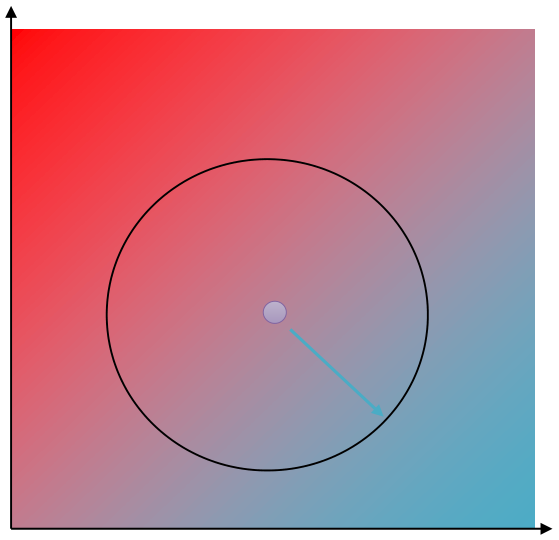
\includegraphics[width=0.8\linewidth]{figures/gradiente.png}
        \caption{Restricción en el caso de descenso por gradiente.}
    \end{subfigure}
    \begin{subfigure}{.45\textwidth}
        \centering
        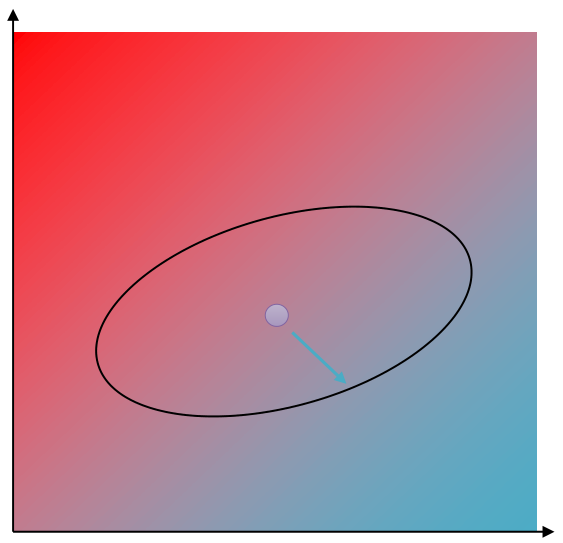
\includegraphics[width=0.8\linewidth]{figures/cuadratica.png}
        \caption{Restricción en el caso de la restricción cuadrática. Se tiene una elipse}
    \end{subfigure}
    \caption{En estas imágenes, se muestra el salto realizado por ascenso por gradiente en la
    dirección ascendente. El color azul indica valores altos y rl rojo valores bajos. Se
puede ver que se está optimizando sobre un plano.}
\end{figure}

En el caso de la elipse, es difícil calcular exactamente donde va a caer el salto al contorno de
la elipse. Por lo que se puede multiplicar al objetivo por $F^{-1}$. Por lo que ahora se puede
optimizar de forma equivalente al nuevo objetivo con el círculo, lo que es mucho más fácil de
calcular.

Por lo que la actualización de los parámetros queda como:
\begin{align}
    \label{eq:naturalgradient}
    \theta'=\theta+\alpha F^{-1}\nabla_\theta J(\theta)
\end{align}
El valor óptimo de $\alpha$ es:
\begin{align}
    \label{eq:trpoalfa}
\alpha = \sqrt { \frac { 2 \epsilon } { \nabla _ { \theta } J ( \theta ) ^ { T } F \nabla _ { \theta } J ( \theta ) } }
\end{align}

Al gradiente de la ecuación \ref{eq:naturalgradient} se le llama \textbf{gradiente
natural}. Se llama así porque este gradiente cambiará la distribución por la misma cantidad sea
cual sea la forma en la que esté representada esa distribución (da igual como esté
parametrizada). 

Como $\theta$ se corresponde a los parámetros del aproximador, en el caso de usar una red
neuronal es posible que $\theta$ sea un vector con millones de parámetros, por lo que para
conseguir una matriz \textit{full-rank} habría que tener el mismo número de muestras. Una
solución a este problema se planteará más adelante.

\subsection{¿Es todo esto necesario?}%
\label{sub:_es_todo_esto_necesario_}

Para comprobarlo, se experimenta con un entorno de prueba.
\begin{figure}[H]
	\centering
	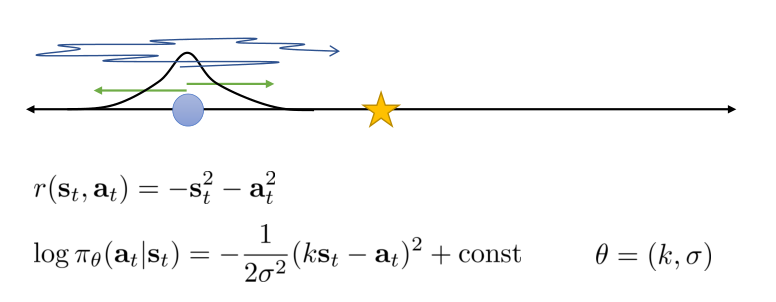
\includegraphics[width=0.8\linewidth]{figures/2020-06-17-165745_776x302_scrot.png}
\end{figure}
Los estados están representados por la recta real negra. El objetivo está en el 0 (representado
por la estrella). El agente es el círculo azul y como acciones puede elegir desplazarse a la
izquierda o a la derecha con valores contínuos. La máxima recompensa se consigue cuando el agente
está en el centro y no toma ninguna acción. La política es una distribución normal, con los
parámetros $\sigma$ y $k$.

Como se tienen sólo dos parámetros, se pueden visualizar los gradientes.

\begin{figure}[H]
	\centering
	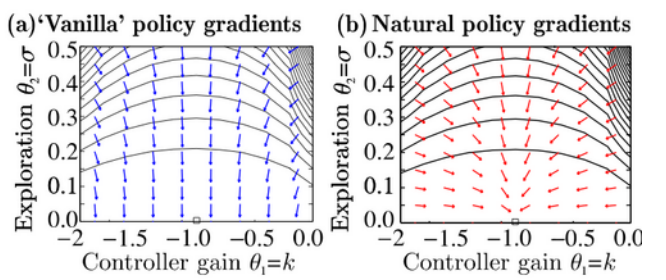
\includegraphics[width=0.5\linewidth]{figures/2020-06-17-170705_666x280_scrot.png}
\end{figure}

Se puede ver que para Policy Gradients normal, los gradientes no llevan al punto óptimo. En
realidad los gradientes de los laterales al punto óptimo están ligeramente inclinados, pero es
apenas perceptible. Esencialmente es el mismo problema encontrado en el descenso por gradiente al
intentar optimizar matrices pobremente condicionadas (elipses muy 'estiradas'), en al que los
parámetros van haciendo zig-zag mientras convergen muy lentamente.

Usando los gradientes naturales, los gradientes llevan directamente al punto óptimo.

\section{Resumen}%
\label{sec:resumen}

\begin{itemize}
    \item Gradiente de la política natural
        \begin{itemize}
            \item Normalmente es una buena opción para estabilizar PG.
            \item Más información en: \textit{Reinforcement Learning of motor skills with
                policy gradients} por Peter, Schaals.
            \item Para hacer una implementación práctica requiere los productos de
                vectores de Fisher. No son triviales de conseguir sin calcular la matriz
                completa (para ello, ver \textit{Trust Region Policy Optimization} por
                Schulman et. al.)
        \end{itemize}
    \item TRPO: básicamente es lo mismo pero se escoge $\alpha$ según la expresión
        \ref{eq:trpoalfa}. Se puede pensar que es como una adaptación de Adam especializado
        en gradientes naturales.
    \item También se puede usar los gradientes duales explicados anteriormente
        (Lagrangiano). Mirar: Proximal Policy Optimization.
\end{itemize}
